\section{Background}

\subsection{UPPAAL}
UPPAAL \cite{UPPAAL_in_a_Nutshell} is a comprehensive tool for modeling, simulation and verification of real-time systems that can be modelled as a network of timed automata. Synchronisation within such system can be realised with shared variables or communication channels. The tool is typically used to implement and verify controllers and communication protocols.

Swarm of robots fits within description of a system that can be modelled using UPPAAL: it is a collection of non-deterministic processes - single robots, that are defined using finite control structure, an algorithm that is transformed into a finite state machine. Swarm has to communicate and this can be achieved using channels or shared variables. Finally, the emergent behaviour is a result of individual robot behaviour which is influenced by the passing time.


\subsection{Timed automata in UPPAAL}
Timed automata in UPPAAL is based on timed automata defined by Rajeev Alur and David Dill in \cite{Automata_For_Modeling_Real-Time_Systems}, defined in Definition \ref{def:automaton}. UPPAAL builds on top of that definition extending the states of the automata with invariants. An invariant is a condition on the clock which controls how long an automaton can remain in the given state. An edge between states can be decorated with a guard, synchronisation action, clock resets and variable assignments. Guard is a condition on the clock or integer variables that needs to be satisfied in order for the transition to be enabled. Synchronisation action is sending a signal to corresponding edge(s) or waiting to receive such a signal in order to synchronise transitions. Clock reset and variable assignment are used to update the state which will be used for edge conditions and determine further transitions. \cite{UPPAAL_in_a_Nutshell}

\begin{definition}[Definition of timed automaton \cite{Automata_For_Modeling_Real-Time_Systems}]

A timed automaton is a tuple $(\Sigma, S, S_0, C, E)$ where:\\
$\Sigma$ - input alphabet;\\
$S$ - finite set of automaton states;\\
$S_0 \subseteq S$ - set of start states; \\
$C$ - finite set of clocks; \\
$E \subseteq S \times S [\Sigma \cup {\epsilon}] \times 2^C \times \Phi(C)$ - set of transitions\\\\
An edge in timed automaton is a tuple $\langle s, s', \sigma, \lambda \delta \rangle$, where:\\
$s$ - origin state;\\
$s`$ - destination state;\\
$\sigma$ - input symbol for the transition;\\
$\lambda$ - set of clocks to be reset with this transition;\\
$\delta$ - condition enabling the transition;\\
\label{def:automaton}
\end{definition}

\subsection{Modeling in UPPAAL}
To explain the process of modeling and verification using UPPAAL, we introduce an example model, presented in Figure \ref{fig:automaton_example}. Description of an example model aims to facilitate understanding the implementation section of this work.
\begin{figure}[H]
\caption{An example UPPAAL model}
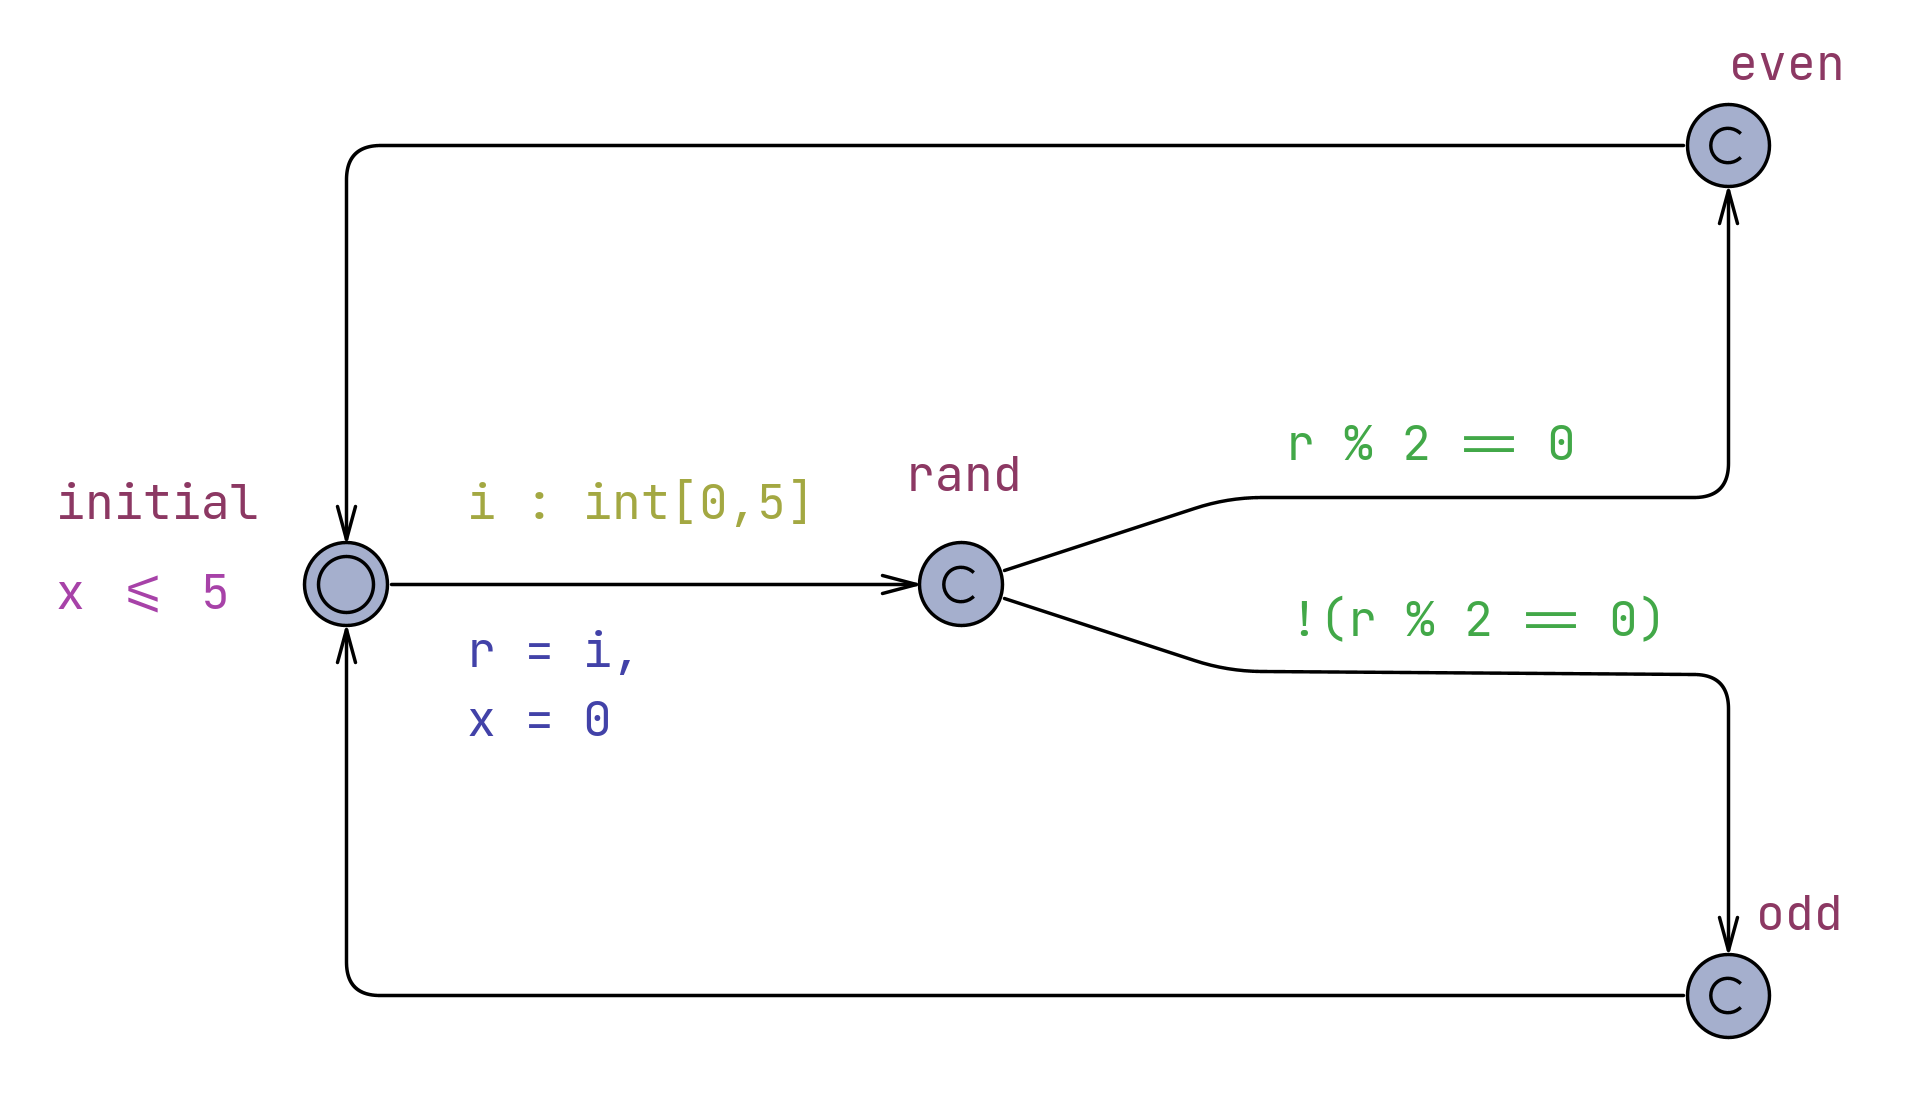
\includegraphics[width=\textwidth]{images/automaton_example.png}
\label{fig:automaton_example}
\end{figure}
\noindent
An example model generates a random integer from the range $[0, 5]$ and classifies it as either an odd or even number, at most every five time units. The model has four locations, namely, initial, rand, even and odd. UPPAAL specifies three types of locations, namely, initial, urgent and committed. Initial location is the starting point of the model. Each model can only have one initial location and in the case of the example model it has the same name as type. If location is of type urgent, the time stops progressing and outgoing transition must be taken immediately. Committed location has all the properties of the urgent location but disallows other models to transition as long as the model is in the committed location. Committed locations are used to build atomic sequences of transitions that cannot be interleaved by other models. Such sequence is created by locations rand, even and odd being of a committed type. The initial location has an invariant on the clock x. The model can remain in the initial location at most five time units. Upon transition from the initial location the clock x is reset. This is achieved by the label associated with the edge that is used for transition. Edge has four possible labels, namely, select, guard, sync and update. Select is used to randomly choose a value from defined range. Guards \texttt{r \% 2 == 0} and \texttt{!(r \% 2 == 0)} hold the logical conditions that need to be satisfied in order to enable transitions. Sync is used for synchronisation between models. Synchronised edge is either waiting for the synchronisation signal to enable the transition or sending it when taking transition. However, this model does not synchronise with any other model as it operates on its own. Update is used for integer variable assignment. In the example model it is used to assign values of two variables, namely, \texttt{r = i} and \texttt{x = 0}.  Transition from the initial location to rand involves selecting integer from the range at random, assigning it to variable and resetting the clock. Edges going from location rand have defined guards, logical conditions that enable transitions. Edge going to location even has condition that checks if the integer drawn at random is even. Edge going to location odd has a condition that is a negation of the condition defined for the edge going to location even. In this way we can guarantee that there will always be only one transition enabled from location rand.

\subsection{Verifying properties in UPPAAL}
UPPAAL uses a subset of timed computation tree logic \cite{Timed_Automata_Semantics_Algorithms_and_Tools} to verify properties of the networks of timed automata .
Properties in UPPAAL are specified using logical quantifiers presented in Definition \ref{def:quantifiers}.

\begin{definition}[Logical quantifiers in UPPAAL \cite{Timed_Automata_Semantics_Algorithms_and_Tools}]
The formulas should be one of the following forms\\
- \texttt{A[]$\phi$} -- Invariantly $\phi$.\\
- \texttt{E<> $\phi$} -- Possibly $\phi$.\\
- \texttt{A<> $\phi$} -- Always Eventually $\phi$.\\
- \texttt{E[] $\phi$} -- Potentially Always $\phi$.\\
- \texttt{$\phi$ --> $\psi$} -- $\phi$ always leads to $\psi$.\\
where $\phi, \psi$ are local properties that can be checked locally on a state, i.e. boolean expressions over predicates on locations and integer variables, and clock constraints.
\label{def:quantifiers}
\end{definition}
\noindent
To check the correctness of implementation of the example model, presented in Figure \ref{fig:automaton_example}, we successfully verified following properties.\\
- \texttt{A[] not deadlock} - model never reaches deadlock.\\
- \texttt{A[] (P.rand || P.odd || P.even) imply P.x == 0} - model in location rand or odd or even, implies that time does not progress.\\
- \texttt{A[] P.even imply (P.r == 0 || P.r == 2 || P.r == 4)} -  model in location even, implies that the integer selected at random is equal to 0 or 2 or 4.\\
- \texttt{A[] P.initial imply P.x <= 5} - model in location initial, implies that elapsed time is smaller or equal than five time units.